\documentclass[a4paper, 11pt,oneside,]{book}
\usepackage{import}
\usepackage[T1]{fontenc}
\usepackage{hyperref}
\usepackage[utf8]{inputenc}
\usepackage{tocloft}
\usepackage[english,italian]{babel} % Lingua principale italiano, con parti in inglese
\usepackage{graphicx} % Per includere immagini esterne
\usepackage[top=3cm,bottom=3cm,left=3cm,right=3cm,headheight=14pt]{geometry} %impaginazione e margini documento
\usepackage{titlesec}
\usepackage{mathptmx} % font simil Times New Roman
\usepackage{fancyhdr}
\usepackage{float}
\usepackage{xcolor}
\usepackage{amsmath}
\usepackage{enumitem}
\usepackage[most]{tcolorbox}

\newtcolorbox{mybox}[2][]{
    title = #2,#1,breakable,
    colback = black!0!white, 
    colframe = black, 
    halign title = flush center,
    fontupper = \itshape,
    fontlower = \itshape,
    segmentation style={solid, black!100}
}

% metainformazioni
\title{Configuratore di auto}
\author{Moretto Mattia}


% personalizzazioni
\graphicspath{{image/}}
\newcommand{\add}[1]{\import{componenti/}{#1}}
\newcommand{\spacing}{\par\bigskip\noindent}

% \titleformat{\chapter}{\bf\huge\scshape}{\thechapter}{1em}{}

\hypersetup{
    colorlinks = false,
    linkbordercolor = black,
    pdfborderstyle = {/S/U/W 1}
}

\pagestyle{fancy}
% fine personalizzazioni



%Inizio Elaborato
\begin{document}

% input file frontespizio.tex
\add{frontespizio}

% Indice
\begingroup
    \hypersetup{hidelinks}
    \tableofcontents
    \addtocontents{toc}{~\hfill\textbf{Pagina}\par}
\endgroup


% Primo capitolo
\chapter{Desiderata}
    \'E richiesto lo sviluppo di un sistema informatico per la vendita online di automobili di un gruppo multi-concessionaria con la possibilità di configurare la versione
    di automobile desiderata.\\
    Il gruppo vende auto di diversi modelli, raggruppati per marca. Per ogni modello di auto il sistema deve poter memorizzare:
    \begin{itemize}
        \item Un nome univoco
        \item Una descrizione
        \item Le dimensioni (altezza, lunghezza, larghezza, peso e volume del bagaglio)
        \item Possibili immagini che permettano di vedere l'auto da vari punti di vista con (potenzialmente diversi colori)
    \end{itemize}
    Il sistema dovrà registrare tutte le ruote a catalogo e definire possibili optional:
    \begin{itemize}
        \item Il colore
        \item Possibili aggiunte
        \begin{itemize}
            \item Ruotino di scorta
            \item Ruota di scorta
            \item Vetro oscurato
            \item Interni in pelle
            \item Ruote con diametri maggiori di quello standard
        \end{itemize}
    \end{itemize}
    Per ogni optional deve essere definito il prezzo e se applicabile o meno al modello scelto.\\
    Per alcuni modelli deve poter essere applicato uno sconto che può variare da un mese all'altro e viene applicato in fase di costruzione del preventivo ed opportunamente 
    indicato. Il cliente deve anche indicare, in caso di acquisto, dove intende ritirare l'auto.
    \spacing
    Un generico utente anche senza autenticarsi deve poter configurare l'auto per la quale pensa di chiedere un preventivo. Successivamente nel momento in cui decide di richiedere
    un preventivo al gruppo è richiesto che l'utente si registri (nel caso in cui non lo fosse già) e poi effetturare l'accesso al sistema. Solo a seguito di ciò avrà quindi la
    possibilità di richiedere la valutazione della sua auto usata allegando delle fotografie.
    \spacing
    Nel caso di valutazione dell'usato, il preventivo verrà finallizato da una persona del negozio, che provvederà a valutare l'usato. Il preventivo potrà essere prodotto anche come file pdf:
    \spacing
    Il sistema memorizza i preventivi effettuati. Entro 20 giorni il potenziale acquirente può confermare il preventivo e pagare un acconto, per ordinare l'auto nella configurazione
    indicata. Il sistema provvederà a proporre una data di consegna (a un mese più 10 giorni per ogni optional richiesto) entro la quale avere l'auto ordinata.
    \spacing
    Il gruppo ha diversi sedi in Italia dov'è possibile ritirare l'auto ordinata. Per ogni sede il sistema deve memorizzare nome, indirizzo completo e tutti gli ordini relativi a quella sede.
    \spacing
    Il sistema deve permettere agli impiegati del gruppo di accedere tramite autenticazione al sistema e gestire i preventivi che richiedono la valutazione dell'usato. Gli impiegati potranno poi 
    gestire gli ordini e avvisare i clienti quando l'auto ordinata è pronta per la consegna (dopo il pagamento dell'iporto dovuto).
    \spacing
    La segreteria amministrativa del gruppo è responsabile dell'inserimento delle informazini su modelli e optional di ogni marca. Essa può accedere al sistema e visualizzare i preventivi per cliente, per marca
    e per negozio di consegna richiesto.
    \spacing
    Il sistema deve inoltre permettere all'utente di configurare l'auto avendo un controllo del prezzo finale dell'auto ad ogni momento.



% Secondo capitolo
\chapter{Specifiche Tecniche}
    \section{Tecnologie utilizzate}
        Di seguito vengono elencate e descritte le principali tecnologie utilizzate per lo sviluppo del software per dare un idea generale di come è composto quanto richiesto. Queste particolari scelte progettuali sono dettate dalla confidenza
        e praticità nell'utilizzo da parte dei componenti del gruppo nell'utilizzarli anche in ambito lavorativo.
        \subsection{C++}
            Si tratta di un linguaggio di programmazione di alto livello orientato agli oggetti e fortemente tipizzato, è stato sviluppato come estensione del linguaggio C ed introdotto negli anni 80.
            C++ combina le caratteristiche della programmazione procedurale con quelle della programmazione orientata agli oggetti, permattendo la creazione di software più complessi, efficienti e modulari.
            \'E ampiamente utilizzato nello sviluppo di sistemi operativi, applicazioni desktop, giochi, software per dispositivi embedded e applicazioni ad alte prestazioni. Grazie alla sua flessibilità e potenza, C++ rimane
            uno dei linguaggi più influenti e utilizzati nel mondo della programmazione.
        \subsection{Angular}
            Angular è un framework open-source per lo sviluppo di applicazioni web, mantenuto da Google e basato su TypeScript, Angular facilita la creazione di applicazioni web dinamiche e reattive grazie alla sua architettura
            a componenti, che consente la suddivisione del codice in moduli riutilizzabili e facilmente gestibili. Tra le sue caratteristiche principali, Angular offre strumenti per il data binding, la gestione delle forme, l'iniezione
            di dipendenze e il routing, semplificando lo sviluppo di applicazioni complesse e scalabili. Grazie alla sua versalità e potenza Angular è una scelta popolare per la creazione di applicazioni web moderne, sia in ambito 
            enterprise che consumer.
        \subsection{Json}
            JSON (JavaScript Object Notation) è un formato leggero per lo scambio di dati, facile da leggere e scrivere sia per le persone che per le macchine. Utilizzato principalmente per trasmettere dati tra un server e un client web, JSON
            rappresenta le informazioni in un formato testuale strutturato basato su coppia chiave-valore, simile ad un oggetto JavaScript. Grazie alla sua semplicità e compatibilità con la maggior parte dei linguaggi di programmazione, JSON è
            diventato uno standard ampiamente adottato per l'interscambio di dati nelle applicazioni web e nelle API. Nel nostro progetto è stato utilizzato come database.
        \subsection{Pistache}
            Pistache è un framework leggero e open-source scritto in C++ per lo sviluppo di server HTTP. Progettato per essere semplice ed efficiente, Pistache offre un architettura basata su eventi e supporta la creazione di server web ad alte prestazioni,
            in grado di gestire numerose connessioni simultanee. \'E particolarmente adatto per lo sviluppo di API RESTfull, grazie alla sua capacità di gestire richieste e risposte HTTP in modo intuitivo e veloce. Pistache è una scelta popolare per gli sviluppatori 
            in C++ che cercano un framework minimalista ma potente per costruire applicazioni web scalabili e performanti.
    \section{Formule applicate}
        Nello sviluppo di questo software ci siamo soffermati su due punti in particolare che richiedevano precise formule per soddisfare la desiderata.
        \spacing
        La prima riguarda la fase di configurazione dell'auto dove il prezzo finale deve sempre essere controllabile in ogni momento pertanto il calcolo che viene fatto è il seguente:
        \begin{gather*}
            p_{f} = p_{0} + {\sum_{0}^{i}} p_{i} \\
            p_{f} = Prezzo \; finale \quad p_{0} = Prezzo \; base \\
            i = Numero \; componenti \; scelti \quad p_{i} = Prezzo \; componente
        \end{gather*}
        Viene omesso il fatto che al prezzo finale ottenuto può essere applicato uno sconto in quanto avverrebbe soltanto in fase di creazione del preventivo e dipende fortemente dal modello e dal periodo dell'ordine
        \spacing
        La seconda invece riguarda la data di consegna entro la quale l'utente puà ritirare l'auto ordinata che deve soddisfare il seguente presupposto:
        \begin{gather*}
            d_{c} > date(now)+(30 + i*10) \\
            d_{c} = data \; consegna \quad i = numero \; componenti
        \end{gather*}
    

            
        

% Terzo capitolo
\chapter{Casi d'uso}
    I casi d'uso permettono di modellare i requisiti funzionali ossia quei requisiti che specificano cosa deve essere fatto. Essi sono indipendenti dalla tecnologia,
    dall'architettura, dalla piattaforma e dal linguaggio di programmazione.\\
    I casi d'uso specificano cosa ci si aspetta da un sistema e allo stesso tempo nascondono come il sistema lo implementa. Sono una sequenza di azioni che producono un risultato osservabile da un attore e vengono utilizzati
    per descrivere i requisiti iniziali (analisi) e a convalidare l'architettura.\\
    Un ottimo elemento per rappresentarli è il diagramma dei casi d'uso che procediamo quindi a sviluppare.
    \section{Diagramma dei casi d'uso}
        Si tratta di un diagramma che esprime un comportamento desiderato o offerto e, solitamente, l'oggetto esaminato è un sistema o una sua parte. Permette di individuare chi o che cosa ha a che fare con il sistema (attore) e cosa
        esso può fare.\\
        Tipicamente il diagramma dei casi d'uso è la prima cosa ad essere creata in un processo o ciclo di sviluppo nell'ambito dell'analisi dei requisiti
        \spacing
        Per comporre correttamente il diagramma dobbiamo prima fare un passo indietro e individuare tutti i casi d'uso che compongono il sistema.
        \spacing
        Per sviluppare i casi d'uso è necessario prima analizzare quella che è la desiderata, ossia, in questo caso, la consegna fornita per lo sviluppo del progetto che è stata riportata nel \hyperlink{chapter.1}{capitolo 1}. Formalizzare i desiderata
        individuando i requisiti è un elemento fondamentale in quanto una specifica errata o incompleta è una delle cause principali del fallimento dei progetti software.
        \spacing
        Procedendo quindi per step andiamo ad analizzare tutto quello che ci viene richiesto, che possiamo riassumere nel seguente modo:
        \begin{itemize}
            \item Software per la vendita di auto (configurabili) online
            \item Un catalogo che prevede diversi modelli raggruppati per marca e con i relativi optional e immagini illustrative
            \item Sconti sui sigoli modelli applicabili e opportunamente indicati in fase di crazione del preventivo
            \item La possibilità per gli utenti che utilizzano la piattaforma di configurare in ogni momento l'auto per cui pensano di richiedere un preventivo anche senza autenticarsi e, previa autenticazione, la possibilità
            di richiedere il preventivo e la valutazione del suo usato
        \end{itemize}
        Lo step successivo è quindi quello di individuare gli attori ossia ruoli che vengono assunti dagli utenti o altre entità che interagiscono col sistema. Un attore deve essere per forza esterno al sistema inoltre non necessariamente deve essere un
        umano. Nello sviluppo del nostro progetto gli attori individuati sono i seguenti:
        \begin{itemize}
            \item Utente/Cliente
            \item Impiegati
            \item Segreteria
        \end{itemize}
        Per ognuno di questi attori è ora possibile individuare i casi d'uso ossia l'obiettivo prefissato all'inzio del capitolo e sono gli elementi che  permettono la creazione del diagramma
        \begin{itemize}
            \item Il cliente consulta il catalogo, si registra e può effettuare acquisti
            \item Il cliente personalizza l'auto
            \item Il cliente richiede un preventivo e sceglie la sede per il ritiro
            \item l cliente può richiedere la valutazione dell'usato
            \item Gli impiegati si autenticano e gestiscono i preventivi che richiedono la valutazione dell'usato
            \item Gli impiegati  gestiscono gli ordini e avvisano quando l'auto è pronta per la consegna
            \item La segreteria si occupa dell'inserimento delle informazioni dei modelli e optional per ogni marca
            \item La segreteria può visualizzare ogni preventivo per cliente, marca e per negozio di consegna
            \item Il cliente paga l'acconto
            \item Il cliente ritira l'auto
        \end{itemize}
        \spacing
        Arrivati a questo punto ci è possibile procedere allo sviluppo del diagramma del caso d'uso collegando innanzitutto i diversi attori ai relativi casi d'uso attraverso le associazioni ossia il primo elemento di collegamento.\\
        Successivamente ci siamo occupati delle diverse dipendenze tra i casi d'uso, nel nostro caso abbiamo deciso di utilizzare:
        \begin{itemize}
            \item \textbf{Include:} dipendenza dove il caso incluso fa parte del comportamento di quello che lo include, si tratta di un comportamento obbligatorio
            \item \textbf{extend:} dipendenza dove il caso d'uso che estende specifica un incremento di comportamento a quello esteso, si tratta di un comportamento opzionale che gestisce casi particolari
        \end{itemize}
        Una volta esserci soffermati su tutti i punti siamo arrivati a creare il diagramma nella sua interezza che si presenta nel seguente modo:
        \begin{figure}[H]
            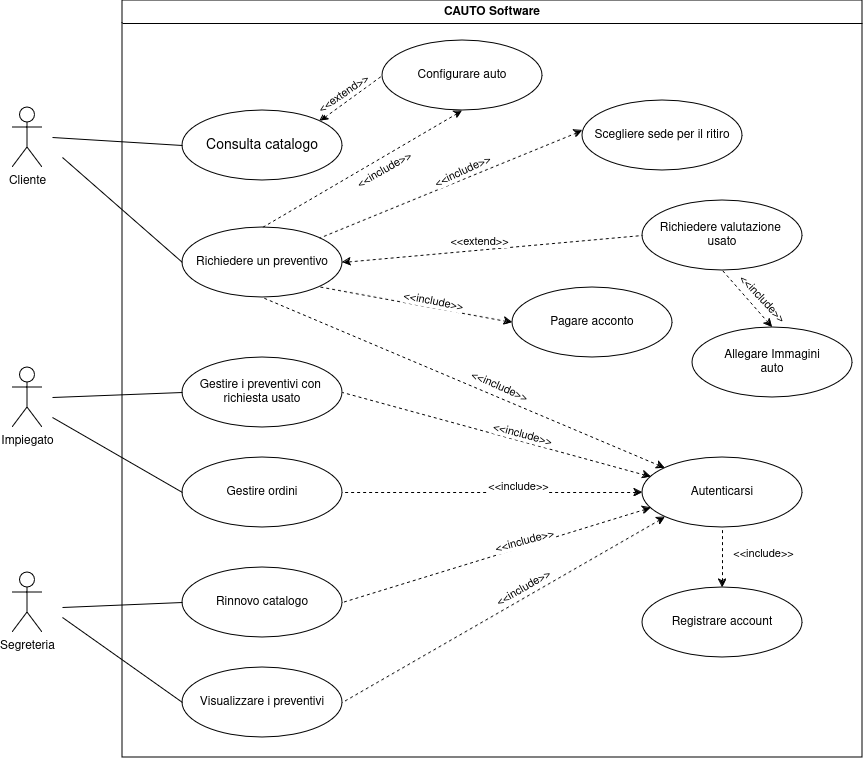
\includegraphics[width=\textwidth]{Diagramma_casi_d'uso.png}
            \caption{Diagramma Casi d'uso}
            \label{fig:diagramma_casi_d'uso}
        \end{figure}
        \spacing
        Quanto riportato è il diagramma d'uso inteso come punto di partenza per lo sviluppo del progetto. Si ha però l'esigenza di abbinare a questo
        diagramma delle specifiche testuali, più formali, in quanto non sono adatti a mostrare la sequenza temporale delle operazioni oppure lo stato del
        sistema e degli attori prima e dopo l'esecuzione. \'E necessario quindi procedere con la descrizione (specifica) dei casi d'uso
    \section{Schede di specifica}
        Ogni caso d'uso ha un nome e una specifica, quest'ultima è composta da:
        \begin{itemize}
            \item \textbf{precondizioni:} condizioni che devono essere vere prima che il caso d'uso di possa eseguire
            \item \textbf{sequenza degli eventi:} i passi che compongono il caso d'uso.
            \item \textbf{postcondizioni:} condizioni che devono essere vere quando il caso d'uso termina l'esecuzione
        \end{itemize}
        Partendo quindi dagli utenti/clienti si procede ad analizzare quelle che sono le schede di specifica che lo riguardano
        \begin{mybox}{Consulta catalogo}
           \textbf{ID:} CU1
           \tcbline
           \textbf{Attori}: Utente
           \tcbline
           \textbf{Precondizioni:} Nessuna
           \tcbline
           \textbf{Sequenza}: 
           \begin{enumerate}
            \item Entrare nella pagina dedicata al catalogo delle auto
            \item Osservare e configurare auto
           \end{enumerate}
           \tcbline
           \textbf{Postcondizioni}: Nessuna
        \end{mybox}
        \spacing
        \'E importante evidenziare il fatto che dal consultare il catalogo non è stata specificata alcuna postcondizione in quanto per come il software è stato
        predisposto un utente generico ha la possibilità di consultarlo senza alcun vincolo. Il caso d'uso appena analizzato lo si può quindi definire un'azione "base"
        prevista dal software.\\
        Si passa quindi ad analizzare il successivo caso d'uso che lo si può considerare quello principale all'interno di quello che è il funzionamento dell'applicazione.
        \begin{mybox}{Richiedere un preventivo}
            \textbf{ID:} CU2
            \tcbline
            \textbf{Attori}: Utente
            \tcbline
            \textbf{Precondizioni:} Essersi Registrato sulla piattaforma
            \tcbline
            \textbf{Sequenza}: 
            \begin{enumerate}
                \item Effettuare l'accesso alla piattaforma
                \item Configurare l'auto che ha intenzione di acquistare
                \item
                \begin{enumerate}
                    \item Richiedere direttamente preventivo
                    \item Richiedere la valutazione del proprio usato 
                \end{enumerate}
                \item Scegliere la sede per effettuare il ritiro dell'auto
                \item Attendere finalizzazione del preventivo
                \item Entro 20 giorni confermare il preventivo
            \end{enumerate}
            \tcbline
            \textbf{Postcondizioni}: Pagare acconto
        \end{mybox}
        \spacing
        Elaborate le schede di specifica legate agli utenti si procede ad analizzare quelle relative agli impiegati
        \begin{mybox}{Gestire i preventivi con richiesta usato}
            \textbf{ID:} CU3
            \tcbline
            \textbf{Attori}: Impiegato
            \tcbline
            \textbf{Precondizioni:} \begin{enumerate}
                \item Un cliente ha richiesto la valutazione dell'auto usata durante la richiesta di un preventivo
                \item Essere registrato alla piattaforma
                \tcbline
            \end{enumerate} 
            \textbf{Sequenza}: 
            \begin{enumerate}
                \item Effettuare l'accesso alla piattaforma
                \item Accedere alla pagina dedicata con la lista dei preventivi da finalizzare
                \item Procedere a valutare l'usato
            \end{enumerate}
            \tcbline
            \textbf{Postcondizioni}: Finalizzare il preventivo
        \end{mybox}
        \spacing
        \begin{mybox}{Gestire ordini}
            \textbf{ID:} CU4
            \tcbline
            \textbf{Attori}: Impiegato
            \tcbline
            \textbf{Precondizioni:} 
                \begin{enumerate}
                    \item Essere registrato alla piattaforma
                    \item Acconto del preventivo pagato dall'utente
                    \item Terminato tempo attesa per la data di consegna
                \end{enumerate} 
            \tcbline
            \textbf{Sequenza}: 
                \begin{enumerate}
                    \item Effettuare l'accesso alla piattaforma
                    \item Accedere alla pagina dedicata con la lista dei preventivi
                    \item Procedere ad avvisare l'utente che l'auto è pronta
                \end{enumerate}
            \tcbline
            \textbf{Postcondizioni}: Consegna l'auto nella sede indicata
        \end{mybox}
        \spacing
        Terminate le schede di specifiche che riguardano gli impiegati si procede con quelle legate alla segreteria
        \begin{mybox}{Rinnovo catalogo}
            \textbf{ID:} CU5
            \tcbline
            \textbf{Attori}: Segreteria
            \tcbline
            \textbf{Precondizioni:} Essere registrato alla piattaforma
            \tcbline
            \textbf{Sequenza}: 
                \begin{enumerate}
                    \item Effettuare l'accesso alla piattaforma
                    \item Accedere alla pagina dedicata con il catalogo delle auto
                    \item Inserimento di informazioni su modelli e optional di ogni marca
                \end{enumerate}
            \tcbline
            \textbf{Postcondizioni}: Nessuna
        \end{mybox}
        \spacing
        Il caso d'uso che riguarda il rinnovo del catalogo è un'azione fine a se stessa, nel senso che si tratta di qualcosa che viene svolto
        dalla segreteria come parte del proprio lavoro, da questa azione non ne consegue nessun'altra ma è importante per avere il catalogo sempre
        aggiornato e influisce sui casi d'uso degli altri attori. Lo stesso vale per la prossima scheda, si potrebbe definire la segreteria come un attore passivo.
        \begin{mybox}{Visualizzare i preventivi}
            \textbf{ID:} CU6
            \tcbline
            \textbf{Attori}: Segreteria
            \tcbline
            \textbf{Precondizioni:} Essere registrato alla piattaforma
            \tcbline
            \textbf{Sequenza}: 
                \begin{enumerate}
                    \item Effettuare l'accesso alla piattaforma
                    \item Accedere alla pagina dedicata con la lista dei preventivi
                    \item Visualizzare i preventivi per cliente, marca e negozio di consegna richiesto
                \end{enumerate}
            \tcbline
            \textbf{Postcondizioni}: Nessuna
        \end{mybox}



%quarto capitolo
\chapter{Diagramma della classi}
    Un diagramma delle classi è un tipo di diagramma utilizzato nella modellazione ad oggetti. Serve per rappresentare la struttura statica di un sistema mostrando le classi, gli attributi, i metodi
    e le relazioni tra di esse come l'ereditarietà, l'associazione e la composizione. Si tratta di uno strumento fondamentale per la progettazione del software poichè consente di visualizzare e definire
    chiaramente l'architettura del sistema, facilitando la comprensione, la manutenzione e l'implementazione del codice.
    \spacing
    Si tratta del secondo step che abbiamo deciso di sviluppare in quanto, una volta ultimato, permetteva una stesura iniziale del codice avendo già ideato quella che doveva essere a grandi linee la 
    struttura dal software.
    \spacing
    All'interno del diagramma ogni classe viene rappresentata in forma di un rettangolo, che può avere fino a 3 slot:
    \begin{itemize}
        \item nome e l'eventuale stereotipo (in UpperCamelCase, obbligatorio)
        \item attributi (in lowerCamelCase, opzionali)
        \item operazioni (in lowerCamelCase, opzionali)
    \end{itemize}
    Ogni classe a sua volta si divide in:
    \begin{itemize}
        \item \textbf{classi di analisi:} solitamente contengono solo quelli più importanti e spesso specificano solo il nome
        \item \textbf{classi di progettazione:} forniscono una specifica completa (implementabile) della classe e dei suoi attributi
    \end{itemize}
    Per rappresentare invece le istanze delle classi si utilizza una notazione molto simile, quinid avranno anch'esse una forma rettangolare. Le differenze sostanziali stanno:
    \begin{itemize}
        \item il titolo degli oggetti è sottolineato e nella forma "nome:classe" con nome opzionale
        \item Non hanno uno slot per le operazioni, possono invece definire valori per gli attributi
    \end{itemize}
%quarto capitolo
\chapter{Diagrammi d'interazione}
    Si tratta di diagrammi di comportamento che modellano le interazioni tra varie entità di un sistema inoltre permettono di visualizzare
    lo scambio di messaggi trà entità nel tempo. Il loro scopo principale è quello di mostrare come un certo comportamento viene realizzato dalla collaborazione
    delle entità in gioco.\\
    Sostanzialmente permette di illustrare il comportamento del sistema da una prospettiva interna inoltre possono avere diversi livelli di astrazione.\\
    Per comporre un diagramma di interazione sono necessarie due cose:
    \begin{itemize}
        \item Un comportamento da realizzare tratto da un classificatore di contesto come per esempio:
        \begin{itemize}
            \item Un caso d'uso
            \item im'operazione di classe
        \end{itemize}
        \item Una serie di elementi che realizzano il comportamento come:
        \begin{itemize}
            \item attori
            \item istanze di classe
        \end{itemize}
    \end{itemize}
    Tutti gli elementi che ci occorrono vengono estrapolati dai vari diagrammi e schede dei capitoli precedenti
\end{document}